\documentclass[../main.tex]{subfiles}

\begin{document}

\begin{theorem}
$\mathcal P(\mathbb H^2)\to\mathbb R$, $[P]\mapsto \mathrm{Area}(P)$ is an isomorphism
\end{theorem}

\begin{proof}

\end{proof}

\begin{theorem}
Suppose $\varphi\in\mathrm{Isom(\mathbb R^2)}$ is rotation by $180^\circ$, $T<\mathrm{Isom(\mathbb R^2)}$ is the translation group, $\mathcal P(\mathbb R^2,\langle T,\varphi\rangle)\cong\mathbb R$
\end{theorem}

\begin{proof}
In Step II of Theorem \ref{P,Q s.c. <=> P,Q have same area}, first we can divide any triangle into triangles with one horizontal side
\begin{center}
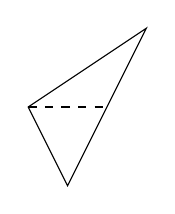
\begin{tikzpicture}[scale=0.5]
\coordinate (a) at (-1,0);
\coordinate (b) at (2,2);
\coordinate (c) at (0,-2);
\coordinate (d) at (1,0);
\draw(a)--(b)--(c)--cycle;
\draw[dashed](a)--(d);
\end{tikzpicture}
\end{center}
The following triangle can be turn into the case in Step II of Theorem \ref{P,Q s.c. <=> P,Q have same area}
\begin{center}
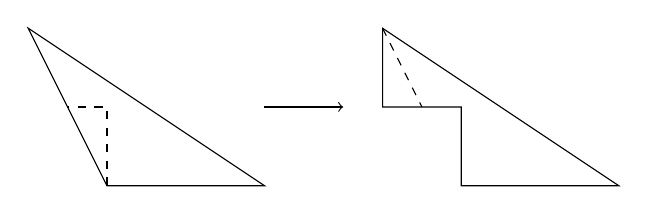
\begin{tikzpicture}
\draw(-1,2)--(0,0)--(2,0)--cycle;
\draw[dashed](0,0)--(0,1)--(-0.5,1);
\draw[xshift=2cm,yshift=1cm,->](0,0)--(1,0);
\begin{scope}[xshift=4.5cm]
\draw(-1,2)--(-1,1)--(0,1)--(0,0)--(2,0)--(-1,2)--cycle;
\draw[dashed](-1,2)--(-0.5,1);
\end{scope}
\end{tikzpicture}
\end{center}
Also, any two congruent rectangle on $\mathbb R^2$ are scissors congruent just by cutting and translating
\end{proof}

\begin{remark}
There is a complete set of invariants needed for $\mathcal P(\mathbb R^2,T)$ called Hadwiger invariants
\end{remark}

\begin{theorem}
$\mathcal P(X)=\mathcal P(X,\mathrm{Isom^+}(X))$, i.e. only orientation preserving isometries are needed
\end{theorem}

\begin{proof}
By Proposition \ref{Conversion of the isometry group in scissors congruence}, $\mathcal P(X)=\mathcal P(X,\mathrm{Isom^+}(X))\otimes_{\mathbb Z[\mathbb Z/2\mathbb Z]}\mathbb Z$ since $\mathrm{Isom}(X)/\mathrm{Isom^+}(X)\cong\mathbb Z/2\mathbb Z$ which is generated by some reflection $r$, we just need to prove $\mathbb Z[\mathbb Z/2\mathbb Z]$ acts trivially on $\mathcal P(X,\mathrm{Isom^+}(X))$ also due to Proposition \ref{Conversion of the isometry group in scissors congruence} \par
As in Lemma \ref{Scissors congruence group is two divisible}, suppose $r_1,r_2,r_3$ are the reflections over $AO$, $BO$, $CO$, and there are $s_i,i=1,2,3$ such that $r_i=s_ig$, then
\begin{align*}
[gP]&=[gP_1]+[gQ_1]+[gP_2]+[gQ_2]+[gP_3]+[gQ_3] \\
&=[s_1gP_1]+[s_1gQ_1]+[s_2gP_2]+[s_2gQ_2]+[s_3gP_3]+[s_3gQ_3] \\
&=[r_1P_1]+[r_1Q_1]+[r_2P_2]+[r_2Q_2]+[r_3P_3]+[r_3Q_3] \\
&=[Q_1]+[P_1]+[Q_2]+[P_2]+[Q_3]+[P_3] \\
&=[P]
\end{align*}
\end{proof}

\begin{definition}\label{Definition of tuple chain complex}
Suppose $X$ is a set, we can define the \textbf{tuple chain complex}\index{Tuple chain complex} $C_*(X)$, where $C_n(X)$ to be the free abelian group generated by $n+1$ tuples $(x_0,\cdots,x_n)$, define the boundary map $\partial:C_n(X)\to C_{n-1}(X)$, $(x_0,\cdots,x_n)\mapsto(-1)^n(x_0,\cdots,\widehat x_i,\cdots,x_n)$
\end{definition}

\begin{lemma}
$H_n(C_*(X))=0$ for $n>0$, i.e. tuple chain complex is acyclic
\end{lemma}

\begin{proof}
Fix $b\in X$, consider $P:C_n(X)\to C_{n+1}(X)$, $(x_0,\cdots,x_n)\mapsto (b,x_0,\cdots,x_n)$, then $\partial P+P\partial=1$
\end{proof}

\begin{definition}
If $X=\mathbb R^n,S^n$ or $\mathbb H^n$, we can defined the convex hull $|(x_0,\cdots,x_n)|$ to be the \textbf{carrier}\index{Carrier} of $(x_0,\cdots,x_n)$, let $C_*^p(X)$ be those tuples such that their carriers lie in a dimension $\leq p$ subspace, note that $C^k_n(X)=C_n(X)$ for $k\geq n$
\end{definition}

\begin{remark}
Note that a $0$-dimensional hyperplane in $S^n$ are antipodal points
\end{remark}

\begin{theorem}
Suppose $X=\mathbb R^n,\mathbb H^n$, then $C_*(X)=C_*^n(X)$, we have an isomorphism $H_n(C_*(X)/C_*^{n-1}(X))\cong\mathcal P(X,\{1\})$
\end{theorem}

\begin{proof}
Define the homomorphism $\varphi:C_n(X)\to\mathcal P(X)$, $(x_0,\cdots,x_n)\mapsto\varepsilon[|(x_0,\cdots,x_n)|]$, $\varepsilon=0$ if $|(x_0,\cdots,x_n)|$ is degenerate, otherwise $\varepsilon=1$ or $\varepsilon=-1$ depending on if the orientation of the carrier matches with $n+1$ tuple $(x_0,\cdots,x_n)$, so by definition, $\varphi$ is really a map $C_n(X)/C^{n-1}_n(X)\to\mathcal P(X)$, $C_n(X)/C^{n-1}_n(X)=Z_n(C_*(X)/C^{n-1}_*(X))$ since $\partial C_n(X)\subseteq C_{n-1}(X)=C_{n-1}^{n-1}(X)$, also 
$\varphi(B_n(C_*(X)/C^{n-1}_*(X)))=\varphi(\partial(C_{n+1}(X)))=\varphi(\partial(C^n_{n+1}(X)))=0$, such as
\begin{align*}
\varphi(\partial(x_0,x_1,x_2,x_3))&=\varphi((x_1,x_2,x_3))-\varphi((x_0,x_2,x_3))+\varphi((x_0,x_1,x_3))-\varphi((x_0,x_1,x_2)) \\
&=[|(x_1,x_2,x_3)|]-[|(x_0,x_2,x_3)|]+[|(x_0,x_1,x_3)|]-[|(x_0,x_1,x_2)|] \\
&=([|(x_1,x_2,x_3)|]+[|(x_0,x_1,x_3)|])-([|(x_0,x_1,x_2)|]-[|(x_0,x_2,x_3)|]) \\
&=[|(x_0,x_1,x_2,x_3)|]-[|(x_0,x_1,x_2,x_3)|] \\
&=0
\end{align*}
\begin{center}
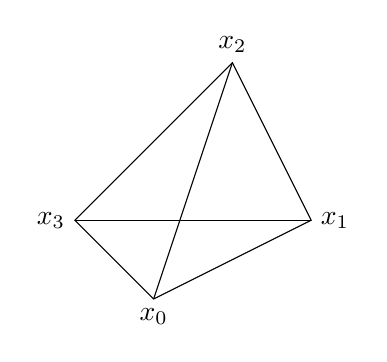
\begin{tikzpicture}
\draw(0,0)--(2,1)--(1,3)--(-1,1)--cycle;
\draw(0,0)--(1,3);
\draw(2,1)--(-1,1);
\node[below] at (0,0) {$x_0$};
\node[right] at (2,1) {$x_1$};
\node[above] at (1,3) {$x_2$};
\node[left] at (-1,1) {$x_3$};
\end{tikzpicture}
\end{center}
Or
\begin{align*}
\varphi(\partial(x_0,x_1,x_2,x_3))&=\varphi((x_1,x_2,x_3))-\varphi((x_0,x_2,x_3))+\varphi((x_0,x_1,x_3))-\varphi((x_0,x_1,x_2)) \\
&=[|(x_1,x_2,x_3)|]+[|(x_0,x_2,x_3)|]+[|(x_0,x_1,x_3)|]-[|(x_0,x_1,x_2)|] \\
&=([|(x_1,x_2,x_3)|]+[|(x_0,x_2,x_3)|]+[|(x_0,x_1,x_3)|])-[|(x_0,x_1,x_2)|] \\
&=[|(x_0,x_1,x_2)|]-[|(x_0,x_1,x_2)|] \\
&=0
\end{align*}
\begin{center}
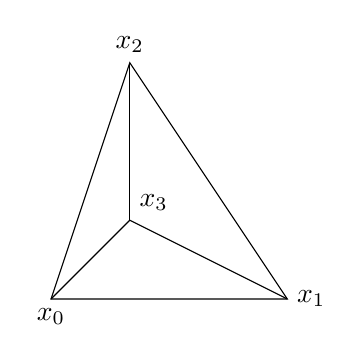
\begin{tikzpicture}
\draw(0,0)--(3,0)--(1,3)--cycle;
\draw(0,0)--(1,1);
\draw(3,0)--(1,1);
\draw(1,3)--(1,1);
\node[below] at (0,0) {$x_0$};
\node[right] at (3,0) {$x_1$};
\node[above] at (1,3) {$x_2$};
\node[above right] at (1,1) {$x_3$};
\end{tikzpicture}
\end{center}
Therefore we get a well-defined map $\varphi:H_n(C_*(X)/C_*^{n-1}(X))\to\mathcal P(X,\{1\})$ \par
We can also define map $\psi:\mathcal P(X,\{1\})\to H_n(C_*(X)/C_*^{n-1}(X))$, $[P]\mapsto (x_0,\cdots,x_n)$, where $x_i$ are the vertices of $P$ that matches up to the orientation
\[\partial(x_0,x_1,x_0,x_2)=(x_1,x_0,x_2)-(x_0,x_0,x_2)+(x_0,x_1,x_2)-(x_0,x_1,x_0)\]
Is equivalent to
\[(x_0,x_1,x_2)=(x_1,x_0,x_2)+(x_0,x_0,x_2)+(x_0,x_1,x_0)+\partial(x_0,x_1,x_0,x_2)\]
Where $(x_0,x_0,x_2)+(x_0,x_1,x_0)+\partial(x_0,x_1,x_0,x_2)=0$ in $H_n(C_*(X)/C_*^{n-1}(X))$ \par
Thus $\psi$ is well-defined, clearly $\varphi$, $\psi$ are inverses to each other, hence $H_n(C_*(X)/C_*^{n-1}(X))\cong\mathcal P(X,\{1\})$ are isomorphic
\end{proof}

\end{document}